\documentclass[11pt]{article}
\usepackage{graphicx}
\usepackage[section]{placeins}
\usepackage{amsmath}

\usepackage[top=1.0in, bottom=1.0in, left=0.5in, right=0.5in]{geometry}
\renewcommand{\thesection}{}
\renewcommand{\thesubsection}{\arabic{subsection}}

\begin{document}
\title{\vspace{15ex}\Huge{Lab07 Report for timing and profiling the code}\vspace{15ex}}


\author{
  Vikas Garg\\120050017\\
  \texttt{vikasgarg@iitb.ac.in}\\[1 cm]
  \and
  Ravi kumar Verma\\120050027\\
  \texttt{ravikumarverma1994@cse.iitb.ac.in}
  \and 
  Dheerendra Singh Rathor\\120050033\\
  \texttt{dheerendra@cse.iitb.ac.in}\\[1 cm]
}

\date{\today}
\maketitle
\newpage
\section{Introduction}
This latex report is targeted towards the study of the timing graphs built in lab05 and the various profiling analysis in this lab.

\section{Timing}
Here we will study the behaviour of the graphs for the timing of the various parts of the code which were generated over 1200 iterations and 20 reruns.
\subsection{Loop Time}
Loop time is the time taken by the for loop in the main.cpp and it is calculated by gettimeofday() method in c++.
\begin{center}
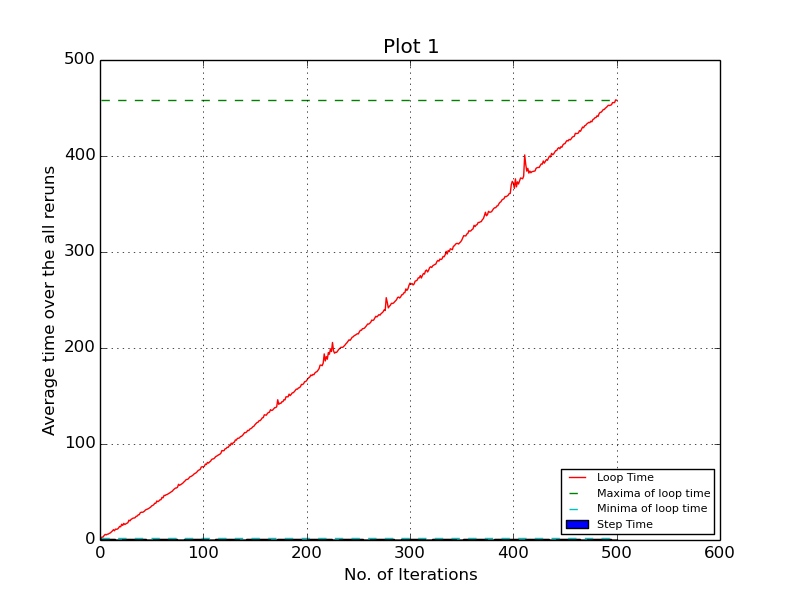
\includegraphics[scale=0.5]{g12_plot01}
\end{center}
As we can see in this graph, the loop is almost linear with respect to iteration value specially on higher iteration values as expected from the system. This graph clearly shows that slop of average loop time vs iteration values is higher for the lower iteration values.
Also step time can be seen very low and close to zero.
\subsection{Other timinings}
Step time is time taken by one step, Collision time is time taken for one collision, Velocity update time is time taken for updating velocity and Position update time is time taken for updating positions.
\begin{center}
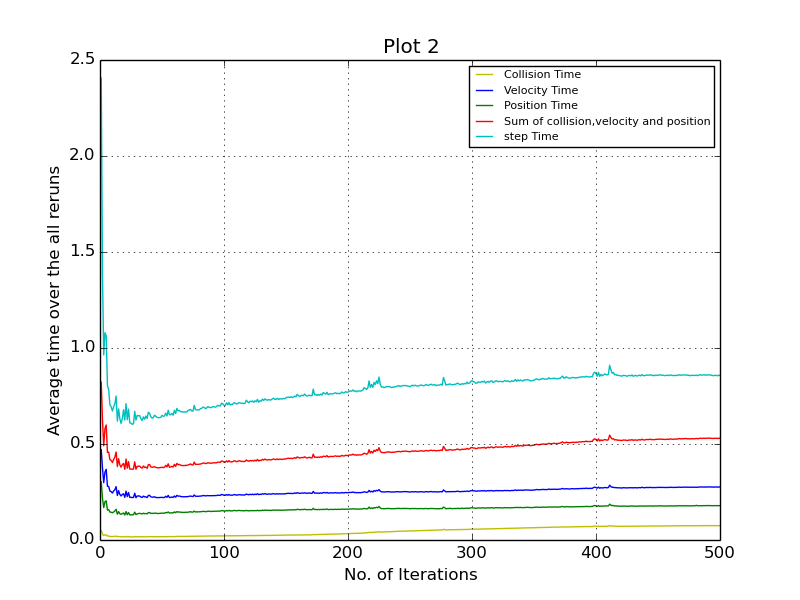
\includegraphics[scale=0.5]{g12_plot02}
\end{center}
From the above graph, we infered following things.
\begin{itemize}
\item Step time is higher than all other times as expected and it is also greater than the sum of collision time, velocity update time and position update time.
\item Other 3 times viz. collision time, velocity update time and position update time are very close to each other.
\item All times have decreased to their minimum till 200 and there is sudden variation in times at 200.There are sudden changes when dominos falls or any other objects interacts.
\end{itemize}
\subsection{Variation over Reruns}
\begin{center}
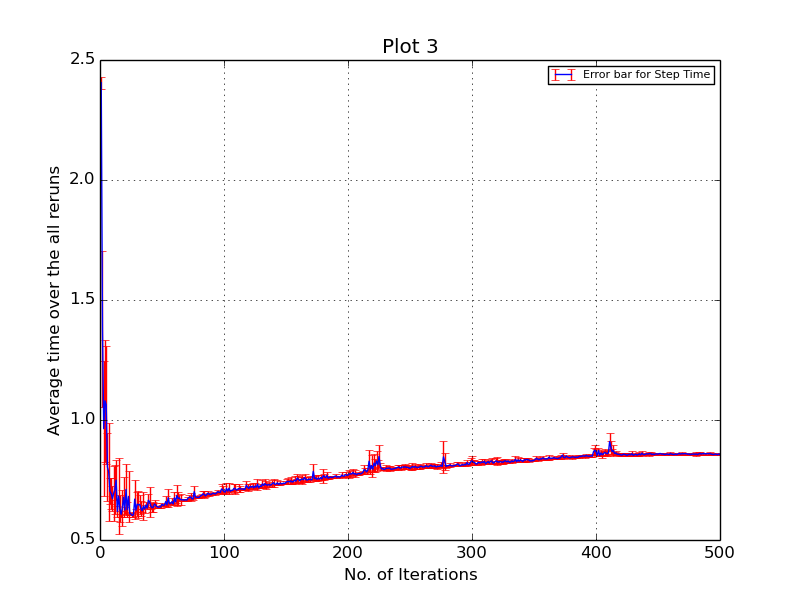
\includegraphics[scale=0.5]{g12_plot03}
\end{center}
As we can see in errorbars graph, there are large variations for different reruns, that are majorly due to different processes running in system and memory available to the main process.\\
Also error decreased with the higher iteration values. except at few points where major interation in the b2world are taking place. And error is more or less proportional to step time.
\subsection{Frequency for fix iteration value}
\begin{center}
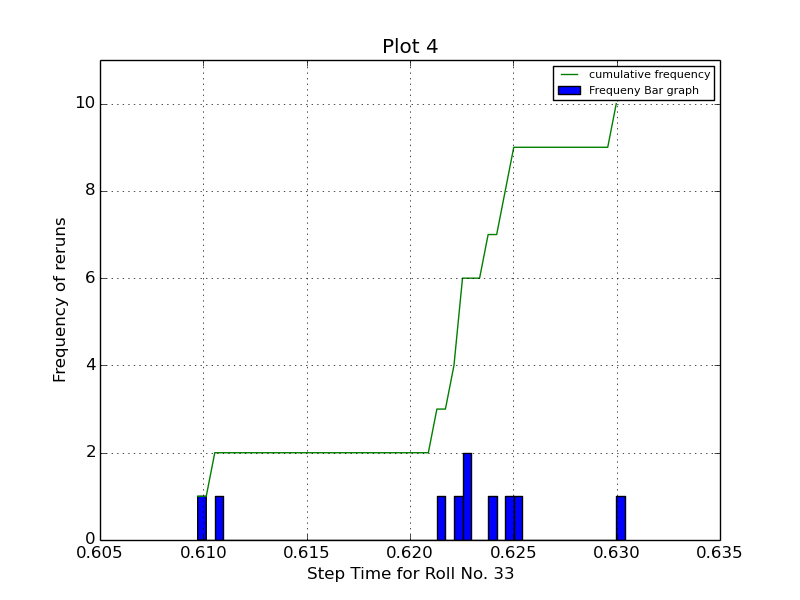
\includegraphics[scale=0.5]{g12_plot04}
\end{center}
Here we chosed the fix iteration value as 33. From the graph we can infer that for low step time frequency is very high that is expected because for a fix iteration value over different reruns the step time should be almost the same. There are some variations in step time also, there are some high values of step times also for the same iteration value.
\subsection{Effect of system load}
when the system is heavily loaded, we can expect that system will slow down due to lack of available memory,  however CPU processes didn't affect the timing as much as memory affects. There is almost no change for small iteration values but for large iteration values the changes are significant.
These differences can not be seen in the graphs due to change in few milliseconds in the loop time.
\subsection{Differece in gettimeofday and time}
Number of Iterations: 10000 \\
Average time per step is 0.040741 ms \\
Average time for collisions is 0.00405339 ms \\
Average time for velocity is 0.0132391 ms \\
Average time for positions is 0.00575907 ms \\
Total loop time is 1285.64 ms \\
real	0m1.302s \\
user	0m1.280s \\
sys	0m0.012s \\

time command gives three different times viz. real, user and sys time. Real time is time from start to finish the call, User is the amount of CPU time spent in user-mode code (outside the kernel) within the process and Sys is the amount of CPU time spent in the kernel within the process. We need to check the user time here. And we can see that user time is slightly greater than total loop time due to the time taken by the other code except for loop. 

\section{Profiling}
Profiling is a form of dynamic program analysis that measures, for example, the space (memory) or time complexity of a program, the usage of particular instructions, or frequency and duration of function calls. The most common use of profiling information is to aid program optimization.\\
Both gprof and perf can be used for profiling, there are several other tools are available on linux too.\\
We have used 'perf' tool for profiling with iteration value 10000.
\subsection{Difference between debug and release mode}
The debug mode will not include optimisations for speed or size and will include additional information such as debugging symbols. Also, in debug mode variables are often set to values that are either sensible or helpful; this will of course entail additional size. Debug mode is used for debugging of programs.\\
The release mode includes optimisation for speed and size and is used for end user product and also includes optimisation in binary product.
\subsection{Release Mode}
for profiling the code in release mode, we installed the Box2D in release mode by using 'cmake -DCMAKE\_BUILD\_TYPE=Release ../'. Also -O3 flag is enabled for release mode.\\
Release mode is using 1k event cycles.\\
\begin{itemize}
\item 25.07\% time is taken by linking libm-2.15.so library and 15.87\% time is taken by libc-2.15.so 
\item b2ContactSolver::SolveVelocityConstrainsts() is taking 7.94\% of total time, we can optimize this function of code to reduce the time.
\item operator+(b2Vec2 const\&, b2Vec2 const\&) is taking 5.05\% time and we can optimise this function also to reducet the time.
\end{itemize}
\subsection{Debug Mode}
for profiling the code in debug mode, we installed the Box2D in release mode by using 'cmake -DCMAKE\_BUILD\_TYPE=Debug ../'. \\
Debug mode is using 4k event cycles.\\
\begin{itemize}
\item 22.13\% time is taken by linking libc-2.15.so library.
\item b2ContactSolver::SolveVelocityConstrainsts() is taking 13.47\% of total time, we can optimize this function of code to reduce the time.
\item operator*(float,b2Vec2 const\&) is taking 9.93\% time and we can optimise this function also to reducet the time.
\item b2Vec2::b2Vec2(float, float) is taking 7.92\% of time and in which 24.39\% of time is taken by operator*(float, b2Vec2 const\&).
\end{itemize}
\subsection{Call Graphs}
call graphs are used for showing interaction between callee and callers, they also shows all functions called with the percentage of time taken shown on arrows.
\subsubsection{Debug Mode}
\begin{center}
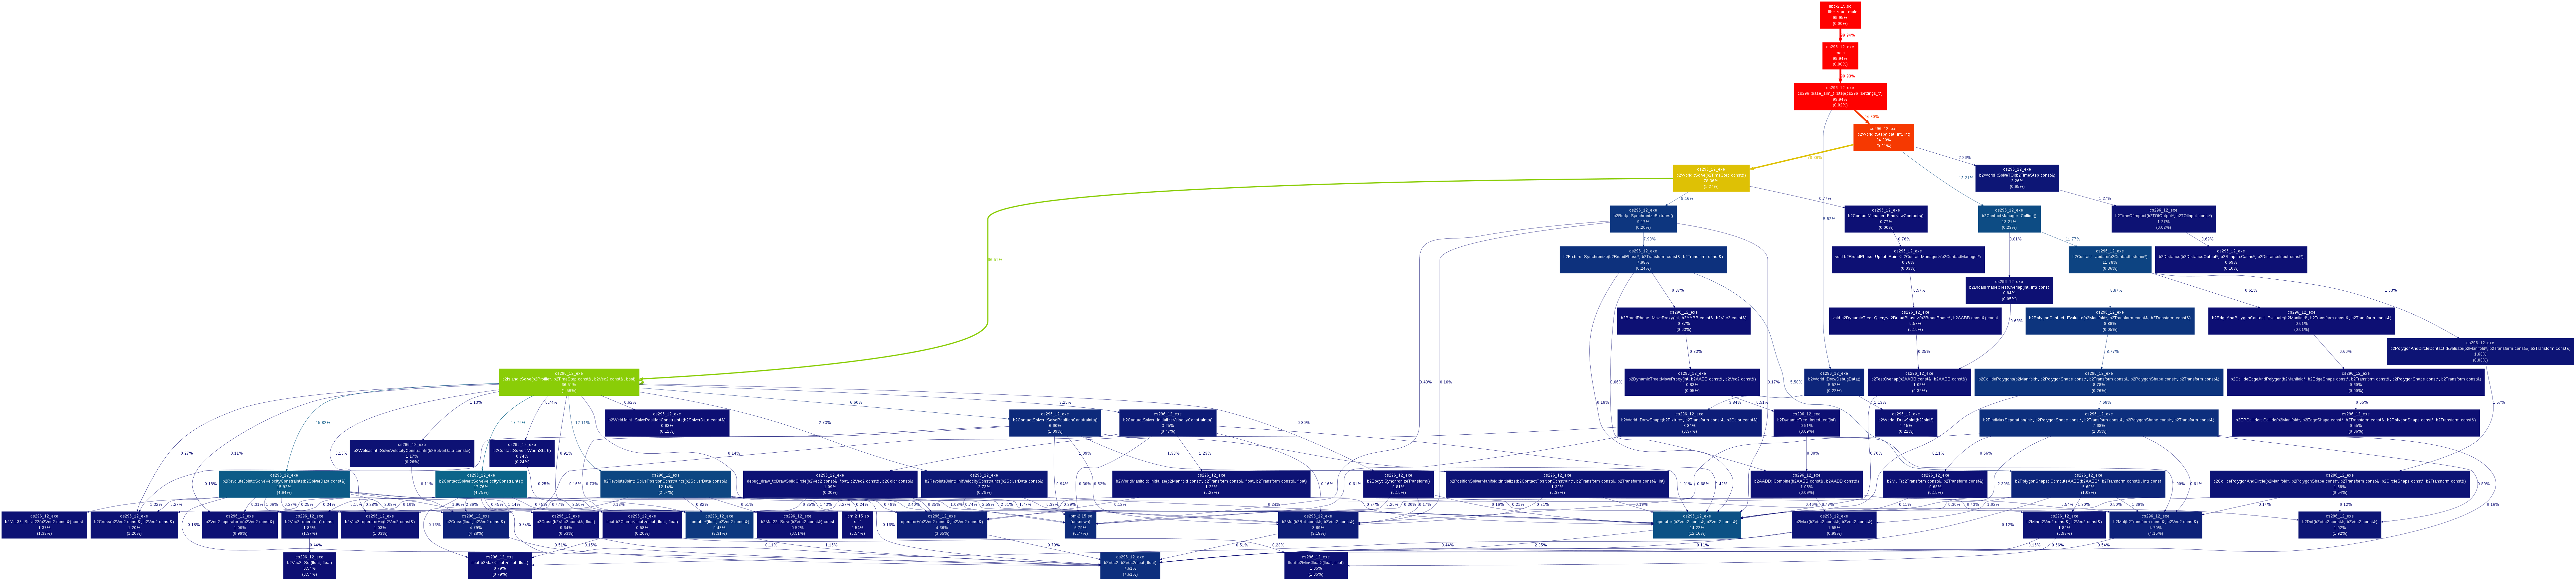
\includegraphics[scale=0.06]{call_graph_debug}
\end{center}
The debug mode has more number of functions calls. Maximum time(96.41\%) is taken by base\_sim\_t function.
\subsubsection{Release Mode}
\begin{center}
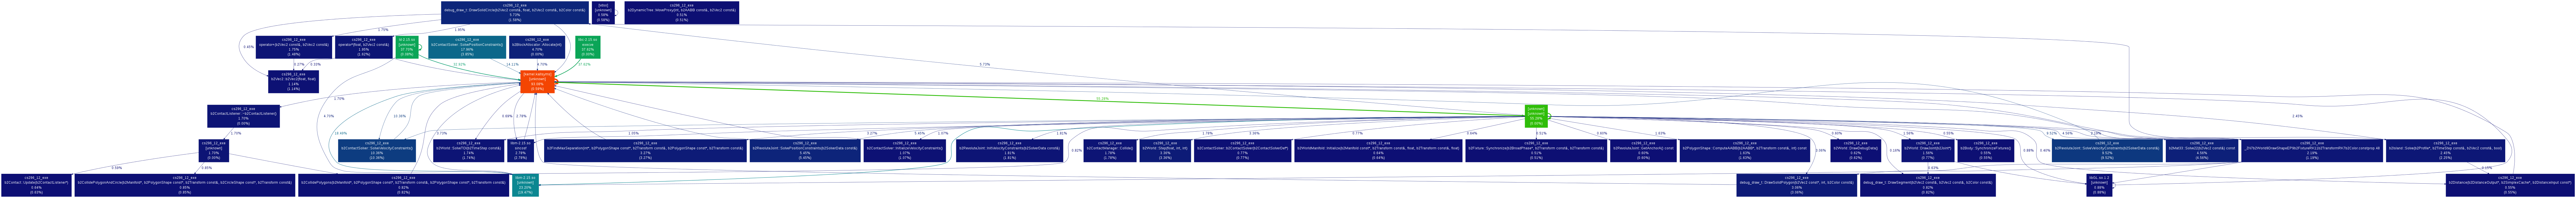
\includegraphics[scale=0.06]{call_graph_release}
\end{center}
The release mode has less number of functions calls because of inline compiling. Maximum time(~34\%) is taken by DrawSolidCircle function.
\end{document}


